\documentclass[11pt]{article}
\usepackage[utf8]{inputenc}
\usepackage{amsmath}
\usepackage{geometry}
\geometry{a4paper, margin=1in}
\usepackage{hyperref}
\usepackage{graphicx}
\usepackage{tikz}
\usetikzlibrary{arrows.meta}
\sloppy % Relax spacing
%\hyphenation{Pressure-Temperature Trade-Offs Nimitz-04} % Commented out to fix "Not a letter" error

\title{One Sun, Three Tricks: Unraveling the Nimitz Enigma}
\author{Max T. Gertz}
\date{February 2025}

\begin{document}
	
	\maketitle
	
	\begin{abstract}
		In November 2004, Navy pilots faced a 40-foot enigma racing at Mach 10. The object had a metal hull and was shaped like a Tic-Tac. Traversing space with ease, it was unmolested by gravity, friction, inertia, and momentum. This was no conjecture—the object was pinned by radar, tracked by FLIR, while Navy pilot David Fravor bore witness. Salvatore Pais offers three Navy patents—fusion’s surge, mass’s slip, gravity’s bend—that might illuminate this enigma. These are grounded in Newton’s laws. Tokamak research, spanning decades, has probed plasma containment depths, while Pais’s patents forge a bold path—potentially unlocking answers plasma physics still seeks. This is no idle fancy; it is a question forged in military data, pursued with scientific reason. Here is how it might fly.
	\end{abstract}
	
	\begin{table}[h]
		\centering
		\small
		\begin{tabular}{|c|l|c|}
			\hline
			\textbf{No.} & \textbf{Equation} & \textbf{Description} \\
			\hline
			\multicolumn{3}{|c|}{\textit{Forces to Negate}} \\
			\hline
			1 & \(F_g = mg\) \cite{newton1687} & Gravitational Force \\
			\hline
			2 & \(F_d = \frac{1}{2} \rho v^2 C_d A\) \cite{bernoulli1738} & Drag Force \\
			\hline
			3 & \(F = ma\) \cite{newton1687} & Inertial Force \\
			\hline
			4 & \(p = mv\) \cite{newton1687} & Momentum's Law \\
			\hline
			\multicolumn{3}{|c|}{\textit{Counter Forces}} \\
			\hline
			5 & \(\nabla \times \mathbf{B} = \mu_0 \mathbf{J}\) \cite{maxwell1865} & Magnetic Field \\
			\hline
			6 & \(\mathbf{F} = q(\mathbf{v} \times \mathbf{B})\) \cite{lorentz1895} & Lorentz Force \\
			\hline
			7 & \(h \propto B E\) \cite{gertsenshtein1962} & Gravity Waves \\
			\hline
			8 & \(F_c = m \omega^2 r\) \cite{newton1687} & Centrifugal Force \\
			\hline
			\multicolumn{3}{|c|}{\textit{Descriptive Extras}} \\
			\hline
			9 & \(\nabla \cdot \mathbf{E} = \rho/\epsilon_0\) \cite{maxwell1865} & Gauss Law \\
			\hline
			10 & \(\mathbf{B} \propto \frac{I}{r^2}\) \cite{biot1820} & Biot-Savart Law \\
			\hline
			11 & \(n \tau E > 10^{20} \, \text{keV·s/m}^3\) \cite{lawson1957} & Lawson Criterion \\
			\hline
		\end{tabular}
		\caption{Table of fundamental equations}
		\label{fig:eqtable}
	\end{table}
	
	\section{Introduction: The Nimitz Enigma}
	Picture November 2004, off the rugged coast of California: Commander David Fravor, seasoned Navy pilot, meets a 40-foot marvel—here dubbed “Nimitz-04” for its Tic-Tac form—cutting Mach 10 through silence. No jets roar, no wings lift; it flips 90 degrees and stops cold, daring four giants—gravity's hold, friction's bite, inertia's heft, momentum's shove—to flinch. Radar traps its form, FLIR catches its steady chill—evidence too stark to deny. By 2017, the sighting breaks free, radar and FLIR footage sparking a fire of wonder. In patent records, Salvatore Pais emerges, his Navy-backed trifecta [2-4]—fusion's surge, mass's slip, gravity's bend—landing near that same year, offering answers where shadows once reigned. This is no mere guess; it is a chase lit by facts, driven by reason.
	
	\subsection{A Curious Feint: The 2005 Patent}
	Two months after Nimitz-04's flight, January 2005, patent US20060145019A1—a “Triangular Spacecraft” [1]—steps forward, oddly timed. Its math glimmers, a scholar's polish, but it falls apart: static fields push nothing, momentum's law flouted—obvious to anyone with physics basics, though the equations might dupe keener UFO fans until they spot the breach.
	\begin{equation}
		p = mv \cite{newton1687}
	\end{equation}
	It posits static fields as thrust, a lure for physics novices dazzled by grand terms like “electrostatic potential”—a cunning 5th generation warfare feint, twisting words to obscure intent. No genius falters so; it is a ruse, baiting dreamers to waste and wander. We discard it, its folly plain, and seize Pais's trio [2-4], Navy-stamped and less suspect—though not immune to doubt. Our method is clear: probe their claims and seek physics flaws, as we did with the woefully ill-advised 2005 sham.
	
	\subsection{Four Fields Nimitz-04 Breaks}
	Fravor saw no illusion. In November 2004, the USS Nimitz crew tracks Nimitz-04—sleek, wingless, flouting physics rules. Radar locks its shape, FLIR catches its steady chill—no heat flares to melt steel or even its Tic-Tac sugar shell; it hits Mach 10, halts sharp, turns at 50g, hovers free. Friction at that speed should sear steel into molten globules, hurled into the Pacific—yet this endures. Its rebellion strikes deep:
	\begin{itemize}
		\item \textit{Gravity}: For centuries, since Newton’s apple in 1666, gravity’s pull—at 9.8 m/s$^2$ pinning all to Earth—has been measured, unyielding across countless trials.
		\begin{equation}
			F_g = mg \cite{newton1687}
		\end{equation}
		A 4,700-cubic-foot steel craft screaming Mach 10 should crash under its own weight---forty tons slamming back to sea in seconds, a flattened wreck on the Pacific floor.\footnote{An ellipsoid (\(\frac{4}{3} \pi \times 20 \times 7.5 \times 7.5\)) yields ~4,700 cubic feet, assuming solid; hollowness varies with wall thickness.}
		\item \textit{Air Friction}: Known since Bernoulli’s 18th-century fluids, friction’s heat scales with,
		\begin{equation}
			F_d = \frac{1}{2} \rho v^2 C_d A \cite{bernoulli1738}
		\end{equation}
		proven by every cannonball and jet to scar the sky. At Mach 10, Nimitz-04’s steel skin—40 feet long—should blister white-hot---liquefying into globs that spray the Pacific, a comet tail of molten ruin.
		\item \textit{Inertia}: Codified by Newton in 1687, inertia binds mass to its path, resisting change with a tyrant’s grip, tested from pendulums to planets.
		\begin{equation}
			F = ma \cite{newton1687}
		\end{equation}
		A 50g turn should rip 4,700 cubic feet of metal apart---bulkheads shearing, hull cracking like an egg, scattering shards over miles of ocean.
		\item \textit{Momentum}: Momentum’s law, conserved since Galileo’s ramps, dictates motion's relentless march, etched in centuries of cannon fire and collisions.
		\begin{equation}
			p = mv \cite{newton1687}
		\end{equation}
		Moving at Mach 10, this steel beast should plow air into a sonic wall---shockwaves blasting a wake, not gliding silent over a sleeping sea.
	\end{itemize}
	This is no campfire yarn—Navy instruments got it dead to rights, no blurry Bigfoot streaking the sky.\footnote{Imagine radar glitching—Mach 10 Sasquatch fleeing the scene, plasma taco in hand [8].} An answer calls, worth the pursuit.
	
	\begin{figure}[h]
		\centering
		\fboxsep=5pt
		\fboxrule=0.4pt
		\fbox{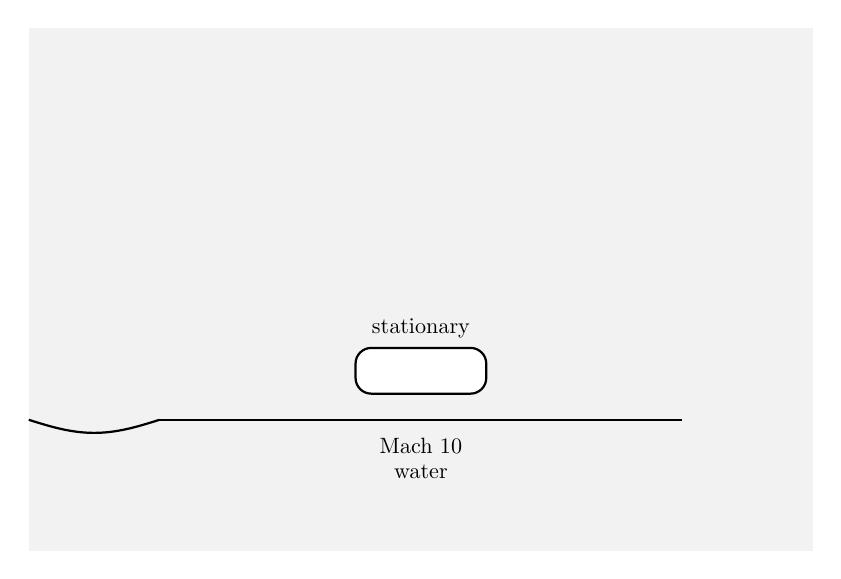
\begin{tikzpicture}[scale=1.66]
				\fill[gray!10] (-1,-1) rectangle (5,3);
				\draw[line width=0.8pt, domain=-1:0, samples=50] plot (\x, {0.1*sin(720*\x/4)});
				\draw[line width=0.8pt, domain=0:4, samples=50] plot (\x, {0});
				\fill[white, rounded corners=0.2cm] (1.5,0.2) rectangle (2.5,0.55);
				\draw[line width=0.8pt, rounded corners=0.2cm] (1.5,0.2) rectangle (2.5,0.55);
				\node[scale=0.8] at (2,0.7) {stationary};
				\node[scale=0.8] at (2,-0.4) {water};
				\node[scale=0.8] at (2,-0.2) {Mach 10};
		\end{tikzpicture}}
		\caption{Tic-Tac hovering over water disturbance}
		\label{fig:water}
	\end{figure}
	
	\begin{figure}[h]
		\centering
		\fboxsep=5pt
		\fboxrule=0.4pt
		\fbox{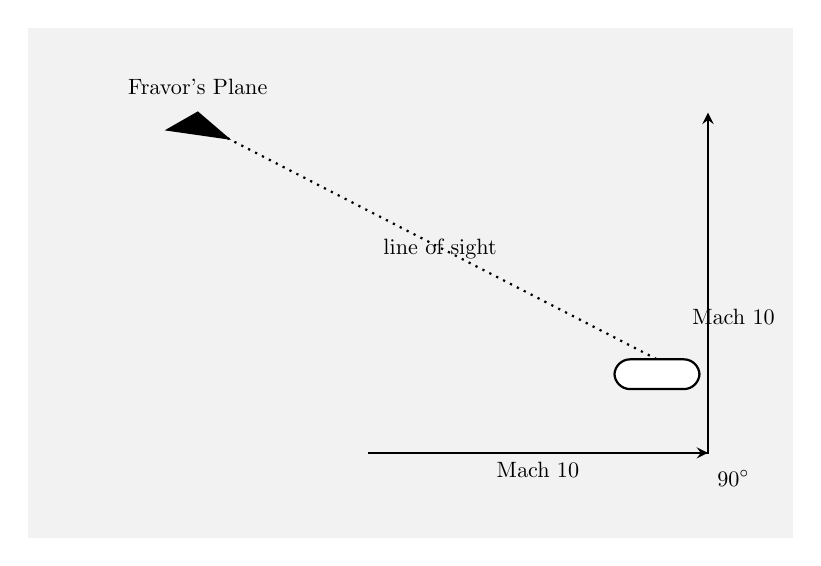
\begin{tikzpicture}[scale=1.08]
				\fill[gray!10] (-4,-1) rectangle (5,5);
				\draw[line width=0.8pt, -stealth] (0,0) -- (4,0) -- (4,4);
				\draw[line width=0.8pt, -stealth] (3.4,0) -- (4,0);
				\fill[white, rounded corners=0.2cm] (2.9,0.75) rectangle (3.9,1.1);
				\draw[line width=0.8pt, rounded corners=0.2cm] (2.9,0.75) rectangle (3.9,1.1);
				\node[scale=0.8] at (4.3,-0.3) {$90^\circ$};
				\fill[black] (-2,4) -- (-2.35,3.8) -- (-1.65,3.7) -- cycle;
				\draw[line width=0.8pt] (-2,4) -- (-2.35,3.8) -- (-1.65,3.7) -- cycle;
				\node[scale=0.8] at (-2,4.3) {Fravor's Plane};
				\draw[line width=0.8pt, dotted] (-1.65,3.7) -- (3.4,1.1);
				\node[scale=0.8] at (0.85,2.4) {line of sight};
				\node[scale=0.8] at (2,-0.2) {Mach 10};
				\node[scale=0.8] at (4.3,1.6) {Mach 10};
		\end{tikzpicture}}
		\caption{Fravor attempts to intercept Nimitz-04}
		\label{fig:intercept}
	\end{figure}
	
	\section{Pais Three Tricks: A Fusion Core}
	
	\subsection{Tokamak Limits and Vibration Promise}
	Tokamaks—pronounced “TacoMax,” no serious person thinks otherwise—wrestle plasma at 100 million degrees Fahrenheit, their toroidal fields coiling to cage fusion fury like a steel tortilla.\footnote{The JET Tokamak peaked at Q approximately 0.7; the ITER Tokamak aims higher—cue the ‘TacoMax’ fiesta, spinning up greasy plasma balls that burst through grilled tortilla walls like Tokamak Tenure on a budget [8]. Q denotes fusion energy gain: output power over input, where Q > 1 yields net energy.} Decades of magnetic confinement—toroidal fields up to 15 tesla—fall short, undone by three flaws. First, stability falters: field wobbles let plasma leak or collapse. Second, containment fails: instabilities (MHD, kink modes) tear plasma loose, scorching walls. Third, energy output lags: Q stalls below 1, power in outpacing power out. A vibrating hull, oscillating at gigahertz [3], offers a fix—atomic agitation to ease fusion, stabilize confinement, and boost yield beyond TacoMax’s limits. This theory, lean and grounded, calls for testing with the means to spark it.
	
	\subsubsection{Counter-Rotation: Taming Plasma’s Fury}
	Vibration alone is not the full fix—counter-rotation steps in where tokamaks falter, two plasma rings, circular and relentless, spinning in opposition to cage what single toroids cannot. Picture them stacked along the Tic-Tac’s spine, one clockwise, one counter, their dance offsetting spin as magnetic fields (\(\nabla \times \mathbf{B} = \mu_0 \mathbf{J}\)) coil tight around each. Tokamaks wrestle one ring’s chaos—kink modes twist, MHD instabilities tear, plasma leaks like a sieve—but here, \textbf{a gyroscopic truce that steadies the storm}. Compression ignites—counter-rotation presses plasma inward—magnetic clash midship—electrostatic field (\(10^6 \, \text{V/m}\)) from vibration squeezes tighter—tames the beast where tokamaks crack. Fusion flares in twin rings—12 capacitors (60 MJ, 0.5 s) boot the spin—x1 (4, 0–0.04 s), x4 (8, 0.04–0.48 s), x1 (2, 0.48–0.5 s)—50–100 MJ output—vibration hums, gigawatts flow—microwave guns birth gravity waves. No torch—self-sustaining—crew safe midship—pressure at 500 bar cuts the temp chase.
	
	\subsubsection{Dual Compression and the Humming Start}
	Stability sets the stage, but containment alone does not ignite—compression lights the fire, and here two forces converge to squeeze plasma into submission. First comes counter-rotation’s dance—two rings churning in defiance—pressing plasma inward as their magnetic fields clash and reinforce, a natural vise that tightens as fusion builds. Second, the electrostatic field, born from the hull’s vibration and the rings’ counter-spun magnetic interplay, scales with the reaction—starting low at 100 kV/m midship, climbing to $10^6$ V/m at the edges as plasma heats to 100 million degrees. This dual grip—rotation’s crush and the field’s squeeze—tames the beast where tokamaks crack, compressing plasma not just to hold it but to spark it. Fusion ignites in both rings, each fed by a capacitor to boot the spin—one per toroid, a twin jolt to kickstart the swirl—then vibration and rotation amplify, feeding on their own energy until the system sings.
	
	Boot-up is the poetry: two capacitors pulse, rings spin, vibration hums low—then fusion flares, magnetic fields surge, and the electrostatic vise clamps harder, all scaling in lockstep. No external torch needed—the craft hums to life, building on itself until gigawatts flow, powering microwave guns that birth gravity waves. Tokamaks dream of this self-sustaining hum; Pais’s trio delivers it—vibration eases the start, counter-rotation holds the line, and compression fuses the impossible. Crew safety seals it: nestled midship, they ride the calm eye as the system roars, a perfect loop of power and control that defies the giants with every pulse. This is no static lab leviathan—fusion’s might, once tethered to sprawling research grids, now roars free in a mobile core, unshackled and unbound. We diverge from Pais here for testability—his terawatt "Pais Effect" [2] awaits future leaps, while our gigawatt fusion leverages current plasma physics for a measurable start.
	
	\vspace{1cm} % Added to prevent "Collision between wrapping environments"
	\begin{figure}[h]
		\centering
		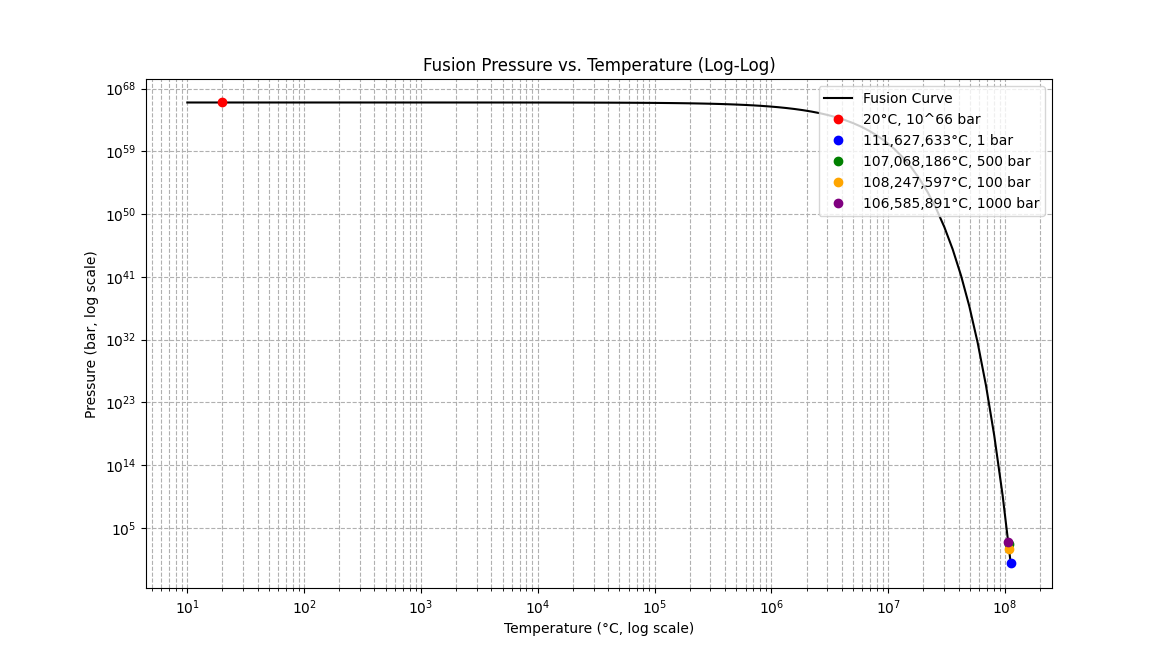
\includegraphics[width=\textwidth]{fusion_curve.png}
		\caption{Fusion Pressure vs. Temperature: Pressure-Temperature Trade-Offs for D-D Fusion}
		\label{fig:flowchart}
	\end{figure}
	
	\subsubsection{Injectors: From Puff to Powerhouse}
	Those injectors don’t just puff hydrogen tangentially—they ignite a cascade that scales from a whisper to a storm, a sub-process as fierce as the fusion it births. It starts with a flick: nozzles, razor-sharp and heat-shielded, blast gas at supersonic snap—say, 3,000 meters per second—into each ring’s curve, a tangential jab that seeds the swirl with a gangster’s cool. Capacitors arc, slamming an electric field—10 kilovts per meter—across the gas, ionizing it into plasma and spinning it into tight vortices, clockwise one ring, counter the other, spiking speeds to $10^5$ meters per second as established physics bends the flow. But the real muscle flexes as fusion sparks: each puff scales with the reaction’s heat—$10^8$ degrees Fahrenheit—ramping pressure and mass flow, injectors pumping harder, plasma thickening until rotation hits millions of meters per second, a cigar-chomping mob boss watching the chaos unfold. This isn’t a static kick; it’s a throttle—vortices meld into a self-feeding surge, locking the rings’ dance tight, ready to power a core that leaves tokamaks in the dust.
	
	\subsubsection{Pressure’s Edge: A Million-Degree Grind}
	Pressure’s brute force—500 bar inner chamber—drops temperature demands by 4.5 million °C from 1 bar’s 111.6 million °C (Fig. \ref{fig:flowchart}). From 500 to 1,000 bar—another 482,000°C shaved—optimization’s game shifts. While Mountain Dew accelerators and queso friars crash in industrial shrines—millions of dollars a pop—a tweak obvious to any air-pressure grunt grinds off degrees—\(Q > 1\) looms—Pais’s fusion [2] meets practical grit.
	
	\subsubsection{Plasma Sheath: Deflecting the Heat}
	Fusion’s fury doesn’t melt the hull—the vibrating hull’s gigahertz hum crafts a plasma sheath, a shield of pure electrostatic might that deflects hot ions before they sear tungsten. At $10^6$ volts per meter, the field’s pressure—\(\epsilon_0 E^2 / 2\)--roaring at $10^9$ newtons per square meter—repels plasma from the walls, a centimeter buffer holding 100 million degrees at bay while the hull idles below 2,000 Fahrenheit. Counter-rotating rings amplify this: their magnetic fields, born of motion, pinch inward at $10^7$ newtons per square meter (\(\frac{B^2}{2\mu_0}\)), bottling heat tighter as fusion scales. No tungsten crumbles, no neodymium drips—this sheath, sparked by vibration and locked by magnetism, turns chaos into order, a containment dance as elegant as Pais’s vision.
	
	\subsubsection{Supercapacitors: The Spark’s Backbone}
	This dance demands juice—supercapacitors, industrial brutes at one cubic meter each, deliver megajoules to spark the storm. Six banks, three per ring, salvo 30 million joules—redundant, relentless, a 99.9999999\% ignition rate—each 5-megajoule shot staged to sustain plasma’s birth, no fizzle allowed. At \$15,000 to \$70,000 apiece, 2025’s tech hands us this scale—grapheme hybrids and hybrid caps shrink the cost, not the dream—fitting a 40-foot hull with room to spare, their weight a whisper against mass reduction’s might. No 1960s room-hoggers here—these are today’s muscle, ready to power fusion’s leap from lab to sky.
	
	\subsubsection{Magnetic Fields from Spinning Plasma}
	Rotation does more than steady the storm—it conjures magnetic might from the plasma’s core, a dynamo born of motion itself. As twin rings whirl—one clockwise, one counter—charged particles, ions and electrons torn from deuterium’s embrace, stream in furious circles, their dance weaving electric currents through the Tic-Tac’s heart. Physics demands it: moving charges birth magnetic fields, a truth etched in the Biot-Savart law \cite{biot1820} and mirrored in the wild spin of stellar disks or lab plasmas. Here, counter-rotation doubles the trick—each ring’s field loops and twists, clashing where they meet to pinch plasma tighter, amplifying as fusion flares and rotation quickens. \textbf{No external coils need linger past the spark; the plasma's own fury sustains the hum}—gigawatts surge, magnetic walls rise, and the hull’s vibration tunes the chaos into order. This is the trifecta’s pulse: fusion feeds the spin, spin feeds the field, and the field locks the giants in a cage of their own making.
	
	\subsection{Stellarator Shapes and Plasma Dynamics}
	Traditional tokamaks confine plasma in a circular torus with unidirectional rotation, using external coils to sustain fusion, as exemplified by reactors like JET and ITER. This theoretically evolves into the stellarator shape of a generic circular craft, where broader toroidal containment employs bidirectional plasma flow for enhanced stability, leading to the Tic-Tac’s ellipsoid design with bidirectional conical streams—fields fully explained in Appendix A—to optimize fusion under extreme conditions.
	
	\subsection{Pais Trifecta: Nullifying the Four Giants}
	Salvatore Pais’s three Navy patents [2-4] do not just hint at Nimitz-04’s flight—they blueprint a machine to crush gravity, friction, inertia, and momentum under one roaring fusion core. Each piece fits, deliberate and fierce, turning the Tic-Tac’s defiance into a puzzle with an answer. Here is how they work together, step by brutal step:
	
	\begin{itemize}
		\item \textit{Fusion Power: The Sun That Fuels It All} \\
		Pais’s fusion device [2] traps a star’s heart—100 million degrees Fahrenheit plasma, far beyond steel’s 2,000 degrees Fahrenheit melt point—inside counter-rotating magnetic rings pinned by
		\begin{equation}
			\nabla \times \mathbf{B} = \mu_0 \mathbf{J} \cite{maxwell1865}
		\end{equation}
		Tokamaks flirt with this; Pais nails it, pumping gigawatts where Q soars past 1. A vibrating hull at gigahertz [3]—think atoms jittering like a TacoMax fryer on Mountain Dew overdrive—stabilizes the plasma, cranks fusion output, and powers the whole show. \textbf{This is not just energy; it is the juice that lets the other two tricks nullify the giants.} Without it, you are grounded.
		
		\item \textit{Mass Reduction: Inertia and Gravity Kneel} \\
		That fusion core feeds a hull wired to hum [3], electric fields rippling at insane frequencies—gigahertz again—to slash the craft’s effective mass with
		\begin{equation}
			\mathbf{F} = q(\mathbf{v} \times \mathbf{B}) \cite{lorentz1895}
		\end{equation}
		Inertia, that stubborn bastard tying mass to its path, fades to nothing; a 50g turn barely nudges the crew, no bones snapping, no steel shredding. Gravity 9.8 m/s$^2$ grip? Same deal—mass drops, and the Pacific floor stays a distant threat. Fusion gigawatts make this hum possible, nullifying two giants in one stroke: inertia is dead, gravity is a ghost.
		
		\item \textit{Gravity Waves: Friction and Momentum Begone} \\
		Fusion’s roar drives microwave pulses [4], fields churning to birth gravity waves—Gertsenshtein’s 1962 trick
		\begin{equation}
			h \propto B E \cite{gertsenshtein1962}
		\end{equation}
		on steroids. These waves do not just ripple; they warp space around the craft, shoving air aside like a bully clearing a path. Friction, the heat that should melt steel at Mach 10, gets no grip—air is displaced before it can claw. Momentum’s relentless march? Canceled—those waves let Nimitz-04 stop cold or flip 90 degrees, no sonic boom, no wake. Fusion powers the pulse; the hull shapes it—leaning on Gertsenshtein’s 1962 prediction \cite{gertsenshtein1962} that EM waves in a magnetic field convert to GWs, not Pais’s resonant cavity [4]. Two more giants bite the dust. \textbf{General Relativity, exhaustively validated across a century of trials, underpins Gertsenshtein's electromagnetic-gravity wave link}—a connection unmeasured not for lack of truth, but for feeble output in prior tests—yet here, bolstered by fusion’s might, we propose a mechanism to amplify those waves into undeniable reality, testing Einstein’s legacy where physics bends but does not break. Replicate this core, and fusion plants could blaze across the globe—compact suns igniting progress; with the reaction live, we turn to tuning, aiming electromagnetic pulses through the field to sculpt gravity waves, their strength no longer a whisper but a roar we must measure.
	\end{itemize}
	
	\subsubsection{Field Geometry’s Role in Gravity Wave Control}
	These giants fall not by chance but by design—gravity waves do not merely emerge, they are sculpted by the field they traverse, a dance of geometry and intent that turns microwaves into spacetime’s reins. Picture the Tic-Tac’s field as a pair of toroidal rings, circular and robust, stretching along its 40-foot hull—unlike the fleeting cones or dishes of theory, these are plasma’s home, shaped by magnetic coils and the hull’s gigahertz hum. This toroidal form, a nod to tokamak lineage, refracts fusion-driven microwave pulses, leveraging Gertsenshtein’s \(h \propto B E\) \cite{gertsenshtein1962} to convert Electromagnetic Waves to Gravity Waves at the $10^6$ V/m boundary—\textbf{we diverge from Pais here for testability--his cavity driven Gravity Waves [4] push theoretical boundaries, while our field refraction builds on Gertsenshtein for near-term proof}—and out they stream, rippling along the hull’s length to part air and silence momentum. Aim matters: point the generators inward, and gravity waves flare outward from midship, a controlled push or pull that shoves the Pacific aside without a whisper—crew safe in the calm eye, far from the emitters’ fury.
	
	A saucer shifts the script—its field a broader torus, hugging the rim of a 40-foot disc. Microwave generators line the edge, firing radially inward toward the core, where the field’s toroidal sweep refracts them into a halo of gravity waves, pulsing outward or tilting with phased intent. Shape dictates destiny: the Tic-Tac’s linear toroids focus waves like a rifle, thrusting forward or halting sharp; the saucer’s radial torus scatters them like a shield, cocooning the craft until steered by emitter tilt. Plausibility lies in this precision—microwaves, gigawatt-strong from fusion’s heart, hit a field tuned to refract, not scatter, their direction set by geometry’s hand. Three patents align here: fusion powers the pulse, vibration shapes the field, and gravity waves ride the form to bury friction’s ghost—a system too cohesive to dismiss.
	
	Together, they are a trifecta of havoc: fusion ignites the engine, mass reduction frees it, gravity waves clear the road. Nimitz-04 does not dodge the four giants—it buries them, fueled by one sun, synced by three beats.
	
	\section{Geometry and Implications: The Craft Takes Shape}
	
	\subsection{A Form Built to Break Rules}
	This trifecta is not abstract—it demands a hull tuned to its chaos. Nimitz-04’s Tic-Tac shape—40 feet long, 15 wide, straight sides, curved ends—channels those fields: fusion spins at the core with
	\begin{equation}
		\nabla \times \mathbf{B} = \mu_0 \mathbf{J} \cite{maxwell1865}
	\end{equation}
	mass-reducing hum coats the skin, gravity waves flare from the tips. Classic UFO discs? Same deal—round rims focus fierce fields, calm centers cradle the crew. \textbf{Call them \textit{Force Gliders} crafts that do not fight physics but work around physics ' limits we are used to obeying,} one sun driving three tricks. This field need not perfectly hug the ship’s contours; it must simply contain Nimitz-04 to work. An oversized field, however, risks perturbing nearby craft during flybys—an effect worth future scrutiny once this concept matures.
	
	\subsection{Crew Safety: Flesh Stays Whole}
	At 50g, flesh should pulp, steel should splinter. Pais’s mass reduction [3] says no—hull vibrations cut inertia and gravity so sharp the crew sips coffee through a Mach 10 turn. Fusion’s steady burn keeps it humming; physics bows, not bodies—\textbf{we diverge from Pais here for testability--his quantum vacuum reduction [3] demands untested exotics, while our vibration and field approach offers a tangible step forward.} Yet inertia reduction alone leaves the crew like feathers in a bowling ball—structurally safe but prone to disruptive motion. The electrostatic field, driven by the toroidal fusion core, compresses the hull with pressures peaking at \(10^6\) V/m near the edges. This field stabilizes the entire craft, ensuring the cabin—nestled in the weaker central field of 100 kV/m—experiences the same relief as the outer structure. The crew avoids chaotic disruption, held steady as the ship defies the giants.
	
	\subsection{Physics We Know, Pushed Far}
	\textbf{this is not sci-fi, it is our toolbox stretched bold.} Maxwell’s 1865 equations [7], Gertsenshtein’s 1962 insight [9], TacoMax’s struggles [8]—Pais patents stack them higher: fusion is real, vibrations tweak it, waves bend space. Labs could test this tomorrow; the Navy’s quiet smirk says they might have already.
	
	\subsection{Conclusion: A Chase Worth Running}
	Nimitz-04 smashed four giants; Pais trio explains how—one sun, three precise strikes. Fusion powers it, mass reduction frees it, gravity waves steer it—Force Gliders rise if we light the spark. Then comes motion—a craft defying gravity’s chains, threading skies with a grace beyond our wildest blueprints. Why is an amateur connecting these dots while tenured heads snooze? Pilots swore it for decades; 2017 gave us radar, FLIR, Fravor’s grit, then patents that might crack it. Yet degreed minds bicker over dogma, crashing TacoMax into molten tortilla heaps instead of chasing data this pure. Curiosity is on life support—wake up, folks, this is not a hoax.
	
	\newpage
	\section*{Appendix A: Field Geometry and the Scaling of Force Gliders}
	The trifecta—fusion core, mass hum, gravity waves—nullifies the four giants through a toroidal field projection, encasing Nimitz-04 in a fixed shell. Unlike tokamaks, the Tic-Tac’s fusion device [2] drives twin ellipsoid plasma flows (16 ft long, 6 ft wide, 4 ft thick, 5 ft apart vertically), mirroring its 40 ft × 15 ft form within a triple containment system. The field’s radius, set by plasma length (\( L_p \)) and hull vibration [3], is calculated as \( R = L_p / 2 + 33 \, \text{ft} \), decaying to Newtonian norms (e.g., 41 ft for \( L_p = 16 \, \text{ft} \)), yielding an 82-ft diameter.
	
	\subsubsection{Field Size Derivation}
	Fusion spins plasma, generating magnetic fields (\(\nabla \times \mathbf{B} = \mu_0 \mathbf{J}\)) [5] from counter-rotating currents. The toroidal field’s extent is fixed by the hull’s gigahertz vibration [3], amplifying the plasma’s dipole-like decay (\(\mathbf{B} \propto 1/r\)) to a baseline distance. For \( L_p = 16 \, \text{ft} \), the field reaches 41 ft from centerline (Appendix A’s original “41 ft out”), where \( R = 16/2 + 33 = 41 \, \text{ft} \). Here, \( D = 33 \, \text{ft} \) is the hull-driven constant from plasma center to boundary, not edge, reflecting vibration and electrostatic amplification (\(10^6 \, \text{V/m}\)). Smaller circuits scale linearly:
	- \( L_p = 1 \, \text{ft} \): \( R = 1/2 + 33 = 33.5 \, \text{ft} \), 67-ft diameter.
	- \( L_p = 2 \, \text{ft} \): \( R = 1 + 33 = 34 \, \text{ft} \), 68-ft diameter.
	- \( L_p = 3 \, \text{ft} \): \( R = 1.5 + 33 = 34.5 \, \text{ft} \), 69-ft diameter.
	This ensures even a 1-ft circuit envelops the 40-ft craft, \( D = 33 \, \text{ft} \) tied to system design, not plasma size alone.
	
	\subsubsection{Containment and Takeoff}
	The ellipsoids, 5 ft apart (centers at \( z = \pm 2.5 \, \text{ft} \)), sit within a single inner chamber (18 ft × 8 ft × 9 ft), dual-walled (1-ft thick), with triple containment: second layer (20 ft × 10 ft × 13 ft) and hull (40 ft × 15 ft × 15 ft), 1-ft air gaps between. Pressure sensors in the inner chamber detect breaches, adjusting symmetric end-vents (fore/aft) during testing to expel heat, preventing flip if one circuit fails. Grounded fusion risks electrostatic grounding (\(10^6 \, \text{V/m}\)), so takeoff uses staged ignition: auxiliary thrusters lift 10 ft, pre-ionization spins plasma (100 kV/m), then full fusion ignites mid-air, scaling fields safely.
	
	\subsubsection{Field Dynamics}
	Field strength scales with fusion intensity, not size, governed by
	\begin{equation}
		\nabla \times \mathbf{B} = \mu_0 \mathbf{J} \cite{maxwell1865}
	\end{equation}
	Electrostatic pressure hits \(10^6\) V/m, the “eye” balances at 100 kV/m (2.5 ft from each center), and gravity waves (\( h \propto B E \)) [4] amplify. A 5-ft hover with an insulated ladder ensures crew exit, the 1-ft gap and 3-ft passages enabling access, with vents and air gaps managing heat in testing. \textbf{This ellipsoid stellarator, unlike the broader disks or compact tokamaks, optimizes containment for the Tic-Tac's unique profile}—future craft may scale it broader or tighter as needed. Sudden landing employs a 5-foot hover with gravity waves [4], dropping an insulated ladder from the eye—no arc, crew clear—though hard contact risks a zap, fusion’s juice potent enough to fry grass, yet the twin-cone toroid ensures hover stability.
	
	\newpage
	\section*{Appendix B: Proposed Methods for Lift and Ignition}
	To lift Nimitz-04 from the ground and ignite its fusion core without grounding electrostatic fields (\(10^6 \, \text{V/m}\)) or destabilizing the craft, three methods emerge, ensuring the system’s viability beyond a blind alley:
	
	\begin{itemize}
		\item \textit{Pre-Lift with Auxiliary Power}: Supercapacitors (30 MJ banks) or chemical thrusters lift the craft 10 ft before fusion starts. Ground clearance prevents arcing, then fusion ignites, engaging mass reduction (\(\mathbf{F} = q(\mathbf{v} \times \mathbf{B})\)) [3] and gravity waves (\(h \propto B E\)) [4] for sustained flight.
		\item \textit{Insulated Launch Platform}: Fusion begins on a dielectric pad (e.g., 10-ft ceramic), delaying grounding. Upward vents expel heat, gravity waves lift off within seconds, avoiding earth discharge.
		\item \textit{Staged Ignition}: Preferred method—auxiliary thrusters lift 10 ft, pre-ionization (100 kV/m) spins plasma via injectors and capacitors, then full ignition (30 MJ) scales fields mid-air. Mass reduction and gravity waves take over, aligning with the 5-ft hover and insulated ladder exit.
	\end{itemize}
	
	These methods mitigate grounding risks, leveraging staged energy release and pre-lift to transition from ground to flight, proving the design’s practical ascent.
	
	\newpage
	\section*{Appendix C: The Triangular Spacecraft—Fool's Gold in a Spook's Faded Briefcase}
	Let us talk about US20060145019A1, the “Triangular Spacecraft” patent from 2005 [1]—a glittering turd dropped two months after Nimitz-04 flew. It has equations, big words like “electrostatic potential,” and a triangle fetish that would make a geometry teacher blush. Sounds legit, right? Wrong. It is a 5th-generation warfare scam, a UFO fanboy trap so dumb it insults the paper it is printed on—and I am here to burn it down.
	
	Start with “electrostatic line charges” on the corners—rear at +V, front at -V, conjuring a “huge horizontal electric field.” I will admit it: first glance, I thought “static electricity”—some wild charge buildup, maybe juiced from the ether like a mad Tesla dream. No. It is just a static electric field—unmoving, ungrooving, a dull voltage slap across a triangle. Not a spark of life, not a hint of recharge—just a fixed potential slumped there like St. Clair’s imagination after a bender. Imagine a prof—say, Dr. Tenure—skimming this, heart racing at “electrostatic,” picturing socks-on-carpet zaps scaled to the stars, only to clock it is an unmoving field. He would chuck his coffee mug at the wall, screaming “Prank!”—and who would blame him? This is not physics; it is a gotcha from a trickster who knew “electrostatic” sounds sexy until you do the math. Momentum's law
	\begin{equation}
		p = mv \cite{newton1687}
	\end{equation}
	yawns—static fields do not thrust, they just sulk.
	
	Then there is the field itself—supposedly uniform, a smooth push from back to front, lifting this tin triangle via EM wave magic. Uniform? Please. Three corners, +V, -V, +V—spin that in your head, and it is a lumpy, irregular mess. Electrostatics 101: point charges make fields that spike near the source, not flat carpets of force. Picture it: a jagged, uneven buzz, strong at the tips, weak in the gaps—nothing uniform about it. J.Q. St. Clair’s banks on you missing that, dazzled by “huge field” hype,
	\begin{equation}
		\nabla \cdot \mathbf{E} = \rho/\epsilon_0 \cite{maxwell1865}
	\end{equation}
	but plug in Gauss and it is a clown show—no lift, no sense. A prof duped by this would hide in his office, mortified he fell for a geometry prank dressed as science.
	
	Compare that to Pais’s trio [2-4]: fusion roaring, twin-triangle toroids humming, gravity waves bending space—real meat, not this vegan tofu nonsense. 2005 is a feint—bait for grant-chasers too starry-eyed to see the con, a distraction from Navy patents that bite. But it is deeper: 5th-generation warfare twists truth, sowing doubt with shiny ghosts. St. Clair is not just a fool; he is a pawn in a game to waste dreamers’ time while the real tech—like Nimitz-04—flies free. This? A footnote for laughs, proof we sift gold from garbage—while the spook with the badge polishes St. Clair’s triangle turd, sipping sake between framing moms and cheating on his wife.
	\newpage
	\begin{thebibliography}{11}
		\bibitem{stclair2004} J. Q. St. Clair, ``Triangular Spacecraft,'' U.S. Patent US20060145019A1, 2004.
		\bibitem{pais2019fusion} S. C. Pais, ``Plasma Compression Fusion Device,'' U.S. Patent US20190295733A1, 2019.
		\bibitem{pais2018mass} S. C. Pais, ``Craft Using an Inertial Mass Reduction Device,'' U.S. Patent US10144532B2, 2018.
		\bibitem{pais2019grav} S. C. Pais, ``High Frequency Gravitational Wave Generator,'' U.S. Patent US10322827B2, 2019.
		\bibitem{newton1687} Newton, I., \emph{Philosophiae Naturalis Principia Mathematica}, 1687.
		\bibitem{bernoulli1738} Bernoulli, D., \emph{Hydrodynamica}, 1738.
		\bibitem{maxwell1865} Maxwell, J. C., ``A Dynamical Theory of the Electromagnetic Field,'' \emph{Philosophical Transactions}, vol. 155, 1865.
		\bibitem{lorentz1895} Lorentz, H. A., ``La théorie électromagnétique de Maxwell et son application aux corps mouvants,'' \emph{Archives Néerlandaises des Sciences Exactes et Naturelles}, vol. 25, 1895.
		\bibitem{gertsenshtein1962} Gertsenshtein, M. E., ``Wave Resonance of Light and Gravitational Waves,'' \emph{Soviet Physics JETP}, vol. 14, 1962.
		\bibitem{biot1820} Biot, J.-B. and Savart, F., ``Note sur le magnétisme de la pile de Volta,'' \emph{Annales de Chimie et de Physique}, vol. 15, 1820.
		\bibitem{lawson1957} Lawson, J. D., ``Some Criteria for a Power-Producing Thermonuclear Reactor,'' \emph{Proceedings of the Physical Society}, vol. 70, 1957.
	\end{thebibliography}
	
\end{document}